\chapter{راه‌حل اکتشافی و توزیع‌شده}\label{chap:4-heuristic_distributed}
\thispagestyle{empty}
\section{مقدمه}
%todo suboptimal persian queuing stability constraint
	در \cref{chap:system_model_centralized_decentralized} مدل سیتم به‌صورت کامل توضیح داده شد، مسئله بهینه‌سازی تبیین شد و در ابتدا به روش متمرکز و سپس به روش غیرمتمرکز بررسی و حل شد. محدودیتی که برای حل مسئله وجود داشت بحث خطی‌سازی آن بود و لازم بود که مسئله حتما به‌صورت خطی باشد.
	 در این فصل سعی می‌شود یک راه‌حل اکتشافی\LTRfootnote{Heuristic} که شبه‌بهینه\LTRfootnote{Sub-optimal} است ارائه و بررسی گردد، مزیت این راه‌حل این است که نیازی نیست مسئله به‌صورت خطی تبیین شود، اما عیب آن نسبت به دو راه‌حل قبلی شبه بهینه بودن آن است. 
	 
	 این راه‌حل اکتشافی مبتنی بر یکی از الگوریتم‌های معروف به نام ویتربی\LTRfootnote{Viterbi} است. در ادامه ابتدا مقدمه‌ای در مورد الگوریتم ویتربی گفته می‌شود، سپس مسئله‌ی اصلی به‌صورتی‌که در این فصل قابل استفاده باشد بازنویسی می‌شود و درنهایت الگوریتم اکتشافی مربوطه کامل و نتایح مربوطه بررسی و با دو راه‌حل قبلی مقایسه می‌شود. 
\section{مقدمه‌ای بر ویتربی}
	 ابتدا لازم است که در مورد الگوریتم ویتربی و نحوه‌ی کار آن صحبت شود. این الگوریتم یک الگوریتم پویا\LTRfootnote{Dynamic}، برای پیدا کردن محتمل‌ترین مسیر از حالت‌های پنهان، با داشتن یک توالی از مشاهدات است. این الگوریتم اغلب در مواردی به‌کار می‌رود که با داشتن یک مدل پنهان مارکف و توالی‌ از مشاهدات، می‌خواهیم بدانیم چه توالی‌ از حالت‌ها (مسیر) این مشاهدات را تولید کرده‌اند. به عبارت دیگر ما دنبال محتمل‌ترین مسیر به‌وجودآورنده مشاهدات در یک مدل پنهان مارکف هستیم. 
	 
	 به عنوان ابتدایی‌ترین پاسخ می‌توانیم تمامی مسیرهای ممکن که مشاهده ما را تولید می‌کنند، پیدا کنیم، سپس با محاسبه احتمال آنها، محتمل‌ترین مسیر را بدست آوریم اما می‌توان نشان داد که پیچیدگی زمانی این راه‌حل نسبت به طول توالی $n$، از اندازه نمایی $(O(a^n))$ است. الگوریتم ویتربی یک راه‌حل ارائه می‌دهد که هزینه محاسباتی آن به صورت خطی با طول توالی افزایش می‌یابد، اصطلاحا هزینه آن از اندازه چندجمله‌ای است. فرم نهایی مسئله را می‌توان بدین صورت نوشت: می‌خواهیم مسیر بهینه‌ای مانند $\displaystyle \pi^* = \arg \max_\pi P(x,\pi)$ داشته باشیم، که در آن $x=(x_1, \dots, x_L)$ یکه توالی از مشاهدات و $\pi = (\pi_1, \dots, \pi_L)$ یک توالی از متغیرهای پنهان باشد. 
	 
	 نحوه‌ی عملکرد این الگوریتم بدین صورت است که مسئله را به صورت یک گراف چندمرحله‌ای\LTRfootnote{Multistage} در نظر می‌گیرد. تعداد مرحله‌\LTRfootnote{Stage}ها برابر است با تعداد مشاهدات و در هر مرحله یکی از مشاهدات مورد بررسی قرار می‌گیرد. در هر مرحله تعدادی حالت\LTRfootnote{State} درنظر گرفته‌می‌شود که هر حالت یک پیشامد ممکن در آن مرحله را بیان می‌کند. حال لازم است که دو مدل تابع هزینه\LTRfootnote{Cost function} تعریف شود یک تابع به عنوان هزینه‌ی بودن در هر حالت در هر مرحله و یک تابع به عنوان هزینه انتقال از یک حالت در یک مرحله به یک حالت دیگر در مرحله بعد است، در واقع این دوتابع به نحوی با یکدیگر ارتباط دارند. در هر مرحله، برای هریک از حالت‌های آن مرحله یک مسیر به عنوان مسیر نجات‌یافته\LTRfootnote{Survived path} تعریف می‌شود که برابر است با مسیری از اولین مرحله تا مرحله فعلی که کمترین هزینه ممکن را دارد. در آخرین مرحله نیز هریک از حالت‌ها یک مسیر نجات‌یافته دارد، در این مرحله حالتی که کمترین هزینه ممکن را دارد، مسیر نجات‌یافته‌اش به عنوان مسیر ویتربی\LTRfootnote{Viterbi path} مشخص می‌شود که این مسیر درواقع پاسخ مسئله است. 
	 %todo a picture about viterbi
\section{راه‌حل اکتشافی}	 
	در این بخش قرار است که باتوجه به مقدمه‌ی گفته شده متغیرهای مربوط به الگوریتم ویتربی را برای مسئله اصلی تعریف کنیم. 
	
	ابتدا صورت مسئله اصلی که به صورت غیرخطی است در \cref{eqn:heuristic:def_optimization_problem} آورده می‌شود. 
	\begin{align}\label{eqn:heuristic:def_optimization_problem}
		& \min \sum_{t \in T}\sum_{e \in E} K_1\pi_ex_{t,e}\lambda_{t,e} + K_2\pi_ex_{t,e} \notag \\
		& + \sum_{t \in T}\sum_{f \in F} K_1\pi_fx_{t,f}\lambda_{t,f} + K_2\pi_fx_{t,f} \notag \\
		& + \sum_{t \in T}\sum_{c \in C} K_1\pi_cx_{t,c}\lambda_{t,c} + K_2\pi_cx_{t,c} \notag \\
		&\text{subj. to}  %todo edit subj to
		\cref{eqn:constraint_load_conservation_computing_nodes}
		\cref{eqn:constraint_request_flow_existence}
		\cref{eqn:constraint_load_managing}\notag \\
		&\cref{eqn:constraint_delay}
		\cref{eqn:constraint_queue_stability}
		\cref{eqn:constraint_load_conservation_sensor_nodes_coupling}
		\cref{eqn:constraint_scalability_coupling}
	\end{align}
	حال لازم است که متغیرهای مربوط به الگوریتم ویتربی متناسب با مسئله‌ ما تعریف شوند، می دانیم که هدف از مسئله ما این است که تعدادی وظیفه به تعدادی گره پردازشی ارسال شوند و هرکدام از این وظیفه‌ها در یک یا چند گره پردازشی، پردازش شوند، با هدف اینکه کل هزینه موجود کمترین حالت ممکن باشد، حال می‌توانیم اینگونه فرض کنیم، که هر وظیفه یک مشاهده است و هر گره پردازشی نیز یک پیشامد است یعنی هر وظیفه را به عنوان یک مرحله در نظر بگیریم و در هر مرحله، هر حالت برابر است با یک گره پردازشی، پس درواقع $l$ حالت مختلف داریم و در نهایت الگوریتم ویتربی باید طوری طراحی شود که مسیر ویتربی نشان‌دهنده این باشد که هر وظیفه در کدام گره پردازش شود یا درواقع مسیر ویتربی کمترین هزینه موجود در شبکه را نشان دهد.
	نکته‌ای که باید مدنظر قرار بگیرد بحث پردازش یک وظیفه در چند گره است، همانطور که قبلا توضیح داده شد، بدین صورت است که هر وظیفه این امکان را دارد که شکسته شود و در دو یا چند گره پردازشی پردازش شود و حداکثر می‌تواند در $N_t$ گره پردازش شود. 
	برای این کار در تعداد مرحله‌های الگوریتم یک تغییر کوچک ایجاد می‌کینم به‌این‌صورت که هر بخش شکسته‌شده از هر وظیفه را یک مرحله درنظر می‌گیریم، پس در نهایت $ \displaystyle L_V=\sum_{t \in T} N_t$ مرحله خواهیم داشت. 
	برای حالت‌های هر مرحله نیز لازم است که یک تغییر کوچک ایجاد شود، برای هر وظیفه در بخش اول حالت‌های ممکن برابر است با همان حالت‌های قبل یعنی $l$ حالت، اما در مورد بخش‌های بعدی از یک وظیفه یک حالت دیگر که حالت صفر $(0)$ نام دارد درنظر گرفته‌می‌شود. تعداد حالت‌های ممکن باتوجه به شماره‌ی مرحله در \cref{eqn:heuristic:def_states} دیده می‌شود. 
	\begin{subequations}\label{eqn:heuristic:def_states}
		\begin{align}
			&Z_n =
			\begin{cases}
			\{0\} \bigcup S, & \text{$u = (n \mod N_t) = 1$} \\
			S,               & \text{در غیر این‌صورت}
			\end{cases}
			,n = 1, \dots, L_V \\
			&S = E \cup F \cup C
		\end{align}
	\end{subequations}
	بنابراین تا اینجای کار تعداد مرحله‌ها و همچنین حالت‌های هر مرحله مشخص شد. در ادامه لازم است که چند تابع مختلف تعریف شود یکی از آن‌ها تابع میزان هزینه انتقال از یک حالت در یک مرحله به یک حالت دیگر در مرحله بعد است. که به صورت \cref{eqn:heuristic:def_tx_cost} تعریف می‌شود. 
	\begin{align}\label{eqn:heuristic:def_tx_cost}
		&\Theta_{n-1,n}^{i,j} = \Gamma_{t,u,j} + \phi_{n-1}^i \\
		&u \in \{1, \dots, N_t\}
	\end{align}
که در \cref{eqn:heuristic:def_tx_cost}، $n$ نشان‌دهنده‌ی مرحله، $u$ نشان‌دهنده‌ی شماره‌ی بخش مربوط به هر وظیفه، که نشان می‌دهد کدام بخش از هر وظیفه قرار است بررسی شود که درواقع برای وظیفه $t$ عددی است بین یک تا $N_t$، $i$ و $j$ نشان‌دهنده‌ی حالت هستند. همچنین $\phi_{n-1}^i$ میزان هزینه‌ی بودن در مرحله $n-1$ و حالت $i$ است. 
	
	در ادامه یک متغیر دیگر تعریف می‌کنیم به نام $T_{n-1,n}^{i,j}$ که نشان‌دهنده‌ی تاخیر سیستم است زمانیکه وظیفه مورد نظر در گره $j$ پردازش شود و الگوریتم ویتربی از حالت $i$ در مرحله قبل به این حالت بیاید. این متغیر در \cref{eqn:heuristic:def_delay_level} تعریف شده‌است. 
	\begin{align}\label{eqn:heuristic:def_delay_level}
		T_{n-1,n}^{i,j} =
		\begin{cases}
			0,				& \text{$j = 0$} \\
			\tau_{t,u,j},  	& \text{در غیر این‌صورت}
		\end{cases}
		,n = 1, \dots, L_V
	\end{align}
	در معادله بالا بعد از مشخص شدن وظیفه و گره پردازشی $\tau$ را به راحتی می‌توان به کمک \cref{eqn:def_delay_final} محاسبه کرد. تنها قسمتی که لازم است در مورد آن صحبت شود مقدار $\lambda$ در \cref{eqn:def_delay_final} است. برای هر وظیفه نرخ کل جریان تولیدی در حسگرها مشخص است که لازم است در طی حل مسئله کل این نرخ تولیدی برای پردازش به دست گره‌های پردازشی برسد، پس در هر مرحله از الگوریتم لازم است که مشخص شود چه حجمی از کل جریان تولید مورد بررسی قرار می‌گیرد، ایده‌ی به کار رفته در الگوریتم به این صورت است که ابتدا فرض می‌شود کل جریان تولیدی مربوط به هر وظیفه در مرحله اول از هر وظیفه بررسی می‌شود و برای ارسال به گره‌ها آماده می‌شود، در صورتیکه در یک مرحله هیچ گره‌ای پیدا نشود که منبع کافی برای پردازش کامل وظیفه را داشته باشد آنگاه، وظیفه شکسته می‌شود، یعنی بخشی از جریان تولیدی برای بخش‌های بعدی از وظیفه در نظر گرفته می‌شود و الگوریتم از اول آن وظیفه دوباره اجرا می‌شود. جزئیات دقیق‌تری درمورد آن‌چه که گفته شد در \cref{alg:heuristic} آمده‌است. 
	
	حال با توجه به متغیرهای تعریف شده برای هر حالت در هر مرحله می‌توان مسیر نجات‌یافته را به صورت \cref{eqn:heuristic:def_survived_path} پیدا کرد. 
	\begin{align}\label{eqn:heuristic:def_survived_path}
		&I_n^j = \arg \min_{i \in XP_n^j} (D_{n-1,n}^{i,j}) \\
		&D_{n-1,n}^{i,j} = \Theta_{n-1,n}^{i,j} + M_k \times (T_{n-1,n}^{i,j} - OD_n^j) \times I(T_{n-1,n}^{i,j} - OD_n^j) \notag \\
		&+M_k \times (\lambda_{t,u,j} - \mu_{t,u,j}) \times I(\lambda_{t,u,j} - \mu_{t,u,j})
	\end{align}	
در \cref{eqn:heuristic:def_survived_path} $D_{n-1,n}^{i,j}$ به عنوان معیار نهایی تصمیم‌گیری برای انتخاب مسیر بین حالت $i$ از مرحله $n-1$ و حالت $j$ از مرحله $n$ درنظر گرفته می‌شود. $I_n^j$ به عنوان شمارنده مسیرنجات‌یافته و $XP_n^j$ به عنوان مجموعه‌ی حالت‌های ممکن از مرحله $n-1$ که منابع کافی جهت ورود به حالت $j$ را دارند، درنظر گرفته‌می‌شود. می‌توان گفت که $XP_n^j \subset Z_{n-1}$، یعنی گره‌هایی که منبع کافی جهت انتقال به حالت جدید را ندارند از کل مجموعه حالت‌های مرحله قبل حذف می‌شوند. $M_k$ به عنوان یک هزینه سنگین در نظر گرفته می‌شود برای حالت‌هایی که تاخیر پردازش در آن‌ها از حداقل تاخیر قابل قبول برای پردازش وظیفه بیشتر است. یک متغیر دیگر به‌نام $OD_n^j$ دیده‌می‌شود، که می‌توان گفت بیانگر تاخیر درخواستی\LTRfootnote{Ordinary delay} برای وظیفه موردنظر است که در \cref{eqn:heuristic:def_ordinary_delay} آورده شده است در این رابطه این تاخیر برابر با میزان تاخیر درخواستی هر وظیفه درنظر گرفته‌شده‌است، درحالیکه می‌توانیم برای اطمینان بیشتر این تاخیر را اندکی کمتر از تاخیر درخواستی وظیفه در آن مرحله در نظر بگیریم که از همگرا شدن الگوریتم اطمینان بیشتری حاصل کنیم. 

	\begin{align}\label{eqn:heuristic:def_ordinary_delay}
		OD_n^j = 
		\begin{cases}
			\infty, & \text{$j = 0$} \\
			\delta_t,& \text{در غیر این‌صورت}
		\end{cases}
	\end{align}
	در هر مرحله از الگوریتم لازم است که مسیر نجات‌یافته را برای هر حالت ذخیره کنیم برای این کار از یک بردار به نام $\Lambda$ استفاده می‌کنیم، که به صورت \cref{eqn:heuristic:def_Lambda} بروزرسانی می‌شود. 
	\begin{align}\label{eqn:heuristic:def_Lambda}
		\Lambda_n^j[u] = 
		\begin{cases}
			\Lambda_n^{I_n^j}[u], & 1 \le u \le n-1 \\
			j, 				& u = n
		\end{cases}
	\end{align}
	در هر حالت پس از مشخص شدن شمارنده مربوط به حالت نجات یافته، مسیر نجات‌یافته برای حالت فعلی برابر است به مسیر نجات‌یافته برای حالت نجات‌یافته، به اضافه‌ی خود حالت فعلی. 

\begin{figure*}[!t]
	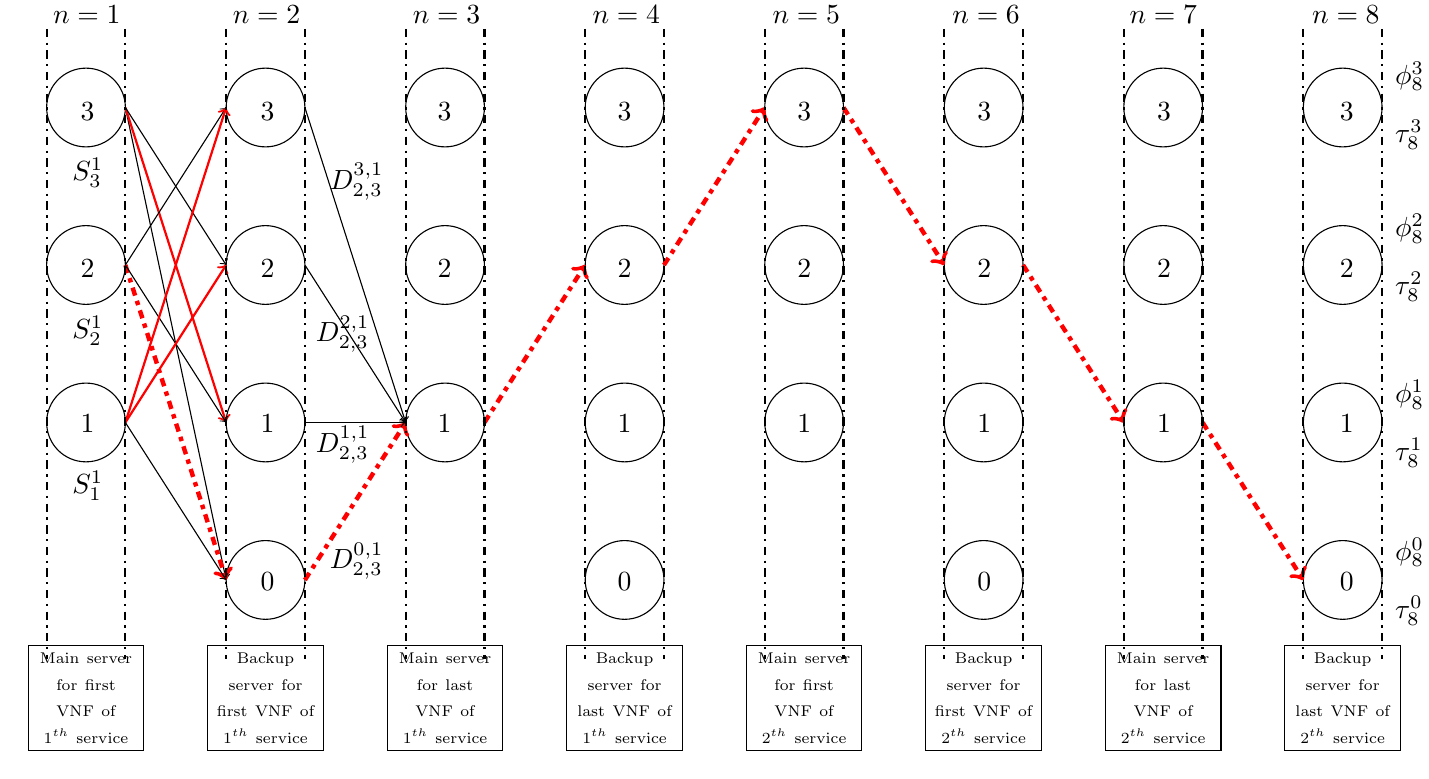
\begin{tikzpicture}[scale=1, every node/.style={scale=0.8}]
	\draw (2,6) circle (0.5cm);
	\draw (2,8) circle (0.5cm);
	\draw (2,10) circle (0.5cm); %%4.2800    6.5600    8.8400   11.1200   13.4000   15.6800   17.9600
	
	\draw (4.28,4) circle (0.5cm);
	\draw (4.28,6) circle (0.5cm);
	\draw (4.28,8) circle (0.5cm);
	\draw (4.28,10) circle (0.5cm);
	
	\draw (6.56,6) circle (0.5cm);
	\draw (6.56,8) circle (0.5cm);
	\draw (6.56,10) circle (0.5cm);
	
	\draw (8.84,4) circle (0.5cm);
	\draw (8.84,6) circle (0.5cm);
	\draw (8.84,8) circle (0.5cm);
	\draw (8.84,10) circle (0.5cm);
	
	%\put(345,168){$\ldots\ldots\ldots\ldots$}
	
	\draw (11.12,6) circle (0.5cm);
	\draw (11.12,8) circle (0.5cm);
	\draw (11.12,10) circle (0.5cm);
	
	\draw (13.4,4) circle (0.5cm);
	\draw (13.4,6) circle (0.5cm);
	\draw (13.4,8) circle (0.5cm);
	\draw (13.4,10) circle (0.5cm);
	
	\draw (15.68,6) circle (0.5cm);
	\draw (15.68,8) circle (0.5cm);
	\draw (15.68,10) circle (0.5cm);
	
	\draw (17.96,4) circle (0.5cm);
	\draw (17.96,6) circle (0.5cm);
	\draw (17.96,8) circle (0.5cm);
	\draw (17.96,10) circle (0.5cm);
	
	\draw [->] (2.5,10) -- (3.78,4);% -- (-10:100pt);
	\draw [->, color=red, thick] (2.5,10) -- (3.78,6);
	\draw [->] (2.5,10) -- (3.78,8);
	
	\draw [->, color=red, ultra thick, dash dot] (2.5,8) -- (3.78,4);
	\draw [->] (2.5,8) -- (3.78,6);
	\draw [->] (2.5,8) -- (3.78,10);
	
	\draw [->] (2.5,6) -- (3.78,4);
	\draw [->, color=red, thick] (2.5,6) -- (3.78,8);
	\draw [->, color=red, thick] (2.5,6) -- (3.78,10);
	
	
	\put(145,255){$D_{2,3}^{3,1}$}
	
	\draw [->, color=red, ultra thick, dash dot] (4.78,4) -- (6.06,6);
	\put(140,200){$D_{2,3}^{2,1}$}
	
	\draw [->] (4.78,6) -- (6.06,6);
	\put(140,160){$D_{2,3}^{1,1}$}
	
	\draw [->] (4.78,8) -- (6.06,6);
	\put(145,118){$D_{2,3}^{0,1}$}
	
	
	\draw [->] (4.78,10) -- (6.06,6);
	
	%% Viterbi path
	\draw [->, color=red, ultra thick, dash dot] (7.06,6) -- (8.34,8);
	\draw [->, color=red, ultra thick, dash dot] (9.34,8) -- (10.62,10);
	\draw [->, color=red, ultra thick, dash dot] (11.62,10) -- (12.9,8);
	\draw [->, color=red, ultra thick, dash dot] (13.9,8) -- (15.18,6);
	\draw [->, color=red, ultra thick, dash dot] (16.18,6) -- (17.46,4);
	
	%% Survived Pathes
	%\draw [->, color=red, thick] (5.5,6) -- (7.5,8);
	%\draw [->, color=red, thick] (5.5,8) -- (7.5,10);
	
	
	
	\draw [thick, dash dot] (1.5,11) -- (1.5,3);
	\draw [thick, dash dot] (2.5,11) -- (2.5,3);
	\node[draw, align = center,text width=1.6cm] at (2,2.5) {\scriptsize{Main server for first VNF of $1^\text{th}$ service}};
	
	\draw [thick, dash dot] (3.78,11) -- (3.78,3);
	\draw [thick, dash dot] (4.78,11) -- (4.78,3);
	\node[draw, align = center,text width=1.6cm] at (4.28,2.5) {\scriptsize{Backup server for first VNF of $1^\text{th}$ service}};
	
	\draw [thick, dash dot] (6.06,11) -- (6.06,3);
	\draw [thick, dash dot] (7.06,11) -- (7.06,3);
	\node[draw, align = center,text width=1.6cm] at (6.56,2.5) {\scriptsize{Main server for last VNF of $1^\text{th}$ service}};
	
	\draw [thick, dash dot] (8.34,11) -- (8.34,3);
	\draw [thick, dash dot] (9.34,11) -- (9.34,3);
	\node[draw, align = center,text width=1.6cm] at (8.84,2.5) {\scriptsize{Backup server for last VNF of $1^\text{th}$ service}};
	
	\draw [thick, dash dot] (10.62,11) -- (10.62,3);
	\draw [thick, dash dot] (11.62,11) -- (11.62,3);
	\node[draw, align = center,text width=1.6cm] at (11.12,2.5) {\scriptsize{Main server for first VNF of $2^\text{th}$ service}};
	
	\draw [thick, dash dot] (12.9,11) -- (12.9,3);
	\draw [thick, dash dot] (13.9,11) -- (13.9,3);
	\node[draw, align = center,text width=1.6cm] at (13.4,2.5) {\scriptsize{Backup server for first VNF of $2^\text{th}$ service}};
	
	\draw [thick, dash dot] (15.18,11) -- (15.18,3);
	\draw [thick, dash dot] (16.18,11) -- (16.18,3);
	\node[draw, align = center,text width=1.6cm] at (15.68,2.5) {\scriptsize{Main server for last VNF of $2^\text{th}$ service}};
	
	\draw [thick, dash dot] (17.46,11) -- (17.46,3);
	\draw [thick, dash dot] (18.46,11) -- (18.46,3);
	\node[draw, align = center,text width=1.6cm] at (17.96,2.5) {\scriptsize{Backup server for last VNF of $2^\text{th}$ service}};
	
	
	%\put(52,260){$\ddots$}\Theta_{n-1,n}^{i,j}
	\put(45,315){$n=1$}
	\put(52,258){$S_{3}^{1}$}
	\put(52,201){$S_{2}^{1}$}
	\put(52,145){$S_{1}^{1}$}
	\put(55,280){$3$}
	\put(55,223){$2$}
	\put(55,167){$1$}
	
	\put(110,315){$n=2$}
	\put(120,280){$3$}
	\put(120,223){$2$}
	\put(120,167){$1$}
	\put(120,110){$0$}
	
	\put(175,315){$n=3$}
	\put(184,280){$3$}
	\put(184,223){$2$}
	\put(184,167){$1$}
	
	\put(240,315){$n=4$}
	\put(249,280){$3$}
	\put(249,223){$2$}
	\put(249,167){$1$}
	\put(249,110){$0$}
	
	\put(305,315){$n=5$}
	\put(314,280){$3$}
	\put(314,223){$2$}
	\put(314,167){$1$}
	
	\put(370,315){$n=6$}
	\put(379,280){$3$}
	\put(379,223){$2$}
	\put(379,167){$1$}
	\put(379,110){$0$}
	
	\put(434,315){$n=7$}
	\put(444,280){$3$}
	\put(444,223){$2$}
	\put(444,167){$1$}
	
	\put(500,315){$n=8$}
	\put(510,280){$3$}
	\put(510,223){$2$}
	\put(510,167){$1$}
	\put(510,110){$0$}
	
	\put(530,293){$\phi_8^3$}
	\put(530,272){$\tau_8^3$}
	\put(530,238){$\phi_8^2$}
	\put(530,217){$\tau_8^2$}
	\put(530,178){$\phi_8^1$}
	\put(530,157){$\tau_8^1$}
	\put(530,121){$\phi_8^0$}
	\put(530,100){$\tau_8^0$}
	
	\end{tikzpicture}
	\vspace{-2mm}
	\caption{An example of using VRSP for placement policy determination in a slot.}
	\label{VRSP_Example}
	\vspace{-4mm}
\end{figure*}

در قسمت بعد لازم است که هزینه‌ی بودن در هر حالت بعد از مشخص شدن مسیر نجات‌یافته بروزرسانی شود. 
\begin{align}\label{eqn:heuristic:def_phi}
	\phi_n^j = \Theta_{n-1,n}^{I_n^j,j}
\end{align}

\begin{latin}
	\begin{algorithm}
		\caption{Heuristic}
		\label{alg:heuristic}
		\begin{algorithmic}[1]
			\State $Z_0 = 0, \phi_0^0 = 0, ResourceIndicator = true, H = L_V, NodeResource_0^0 = \sigma.$ 
			\For{$n=1:L_v$}\label{eqn:alg_steps:heuristic_main_loop}
			\State{Determine the index of considered task, $t$, the index of considered part of task, $u$.}
			\State{Determine the set of states $Z_n$ using \cref{eqn:heuristic:def_states}}
			\State $RemovedStates=\{\}, RepeatIndicator = false$
			\If{u = 1}
			\State update backups
			\EndIf	
			\For{$j\in Z_n$}
			\State $XP_n^j=Z_{n-1}, OD_n^j = \infty$
			\If{$j\neq 0$}
			\For{$i \in XP_n^j$}
			\If{$NodeResource_{n-1}^i < f_t^r(\lambda_{t,u,j})$}
			\State $XP_n^j = XP_n^j - \{i\}$
			\EndIf
			\EndFor
			\State $OD_n^j = \delta_t$
			\EndIf
			\If{$XP_n^j \neq \emptyset$}
			\For{$i \in XP_n^j$}
			\State{Calculate $T_{n-1,n}^{i,j}$ using \cref{eqn:heuristic:def_delay_level}}
			\State Calculate $\Theta_{n-1,n}^{i,j}$ using \cref{eqn:heuristic:def_tx_cost}
			\EndFor
			\State{Calculate $I_n^j$ using \cref{eqn:heuristic:def_survived_path}and $\Lambda_n^j$ using \cref{eqn:heuristic:def_Lambda}}
			\State{Calculate $\phi_n^j$ using \cref{eqn:heuristic:def_phi}}
			\If{$j\neq 0$}
			\State $NodeResource_n^j = NodeResource_n^j - f_t^r(\lambda_{t,u,j})$
			\EndIf
			\Else
			\State $RemovedStates = RemovedStates + \{j\}$
			\EndIf
			\EndFor
			\If{$|RemovedStates| > 0.7 |Z_n|$}
			\State $numOfIters[n] = numOfIters[n] + 1$
			\If{$numOfIters[n] < 7$}
			\State $RepeatIndicator = true$
			\State divide $\lambda_{t,u,j}$ into smaller pieces.
			\State update parameters with backup data.
			\State \textbf{break}
			\EndIf
			\EndIf
			\algstore{myalg}
		\end{algorithmic}
	\end{algorithm}
\end{latin}
\begin{latin}
	\begin{algorithm}                     
		\begin{algorithmic} [1]              
			\algrestore{myalg}
			\If{$RemovedStates = Z_n$}
			\State{Set $H=\sum_{m=1}^{t}{N_m}$ and $ResourceIndicator=false$}
			\State{Determine the Viterbi path $P$, using \cref{eqn:heuristic:def_viterbi_path} with $H$.}
			\State\textbf{break}
			\Else
			\State{Remove all states in the $RemovedStates$ from the $Z_n$}
			\EndIf
			\EndFor
			\If{$RepeatIndicator = true$}
			\State go to \cref{eqn:alg_steps:heuristic_main_loop}, repeat the loop from first part of last task.
			\EndIf
			\If{$ResourceIndicator = true$}
			\State{Determine the Viterbi path $P$, using \cref{eqn:heuristic:def_viterbi_path} with $H$.}
			\EndIf
			\State{Determine the task scheduling using Viterbi path $P$}
		\end{algorithmic}
	\end{algorithm}
\end{latin}

	در آخر لازم است که در هر مرحله بتوانیم مسیر ویتربی را بیابیم، فرض کنیم که در مرحله $\displaystyle H = \sum_{t \in T}N_t$ هستیم، در میان مسیرهای نجات یافته در این مرحله، مسیر ویتربی را می‌توان به کمک \cref{eqn:heuristic:def_viterbi_path} یافت.
\begin{subequations}
	\begin{align}\label{eqn:heuristic:def_viterbi_path}
		&P = \Lambda_H^\zeta \\
		&\zeta = \arg \min_{i \in Z_H} \phi_H^i \times M_k
		%todo correct this fucking formula
	\end{align}
\end{subequations}
در حالتی‌که الگوریتم به خوبی تمام شود و تمام مراحل پیموده شوند می‌توان گفت که $H=L_V$.
\begin{latin}
	\begin{algorithm}
		\caption{Viterbi Path Scheduling}
		\label{alg:viterbi_path_scheduling}
		\begin{algorithmic}[1]
			\For{ i = 1 : H}
			\State{Determine the index of considered task, $t$, the index of considered part of task, $u$.}
			\State{Determine the index of considered computational node n}
			\If{$\tau_{t,u,n} \le \delta_t$}
			\State $x_{t,n} = 1$
			\State $\lambda_{t,n} = \lambda_{t,u,n}$
			\EndIf
			\EndFor
		\end{algorithmic}
	\end{algorithm}
\end{latin}

\section{راه‌حل توزیع‌شده}

در این بخش قرار است که یک روش دیگر برای حل مسئله اصلی استفاده شود. در این روش قرار است که مسئله بهینه‌سازی به‌طور کامل شکسته شود و به صورت توزیع‌شده حل شود. برای این‌کار از الگوریتم ارائه شده در \cite{testa2019distributed} استفاده می‌شود. همانند راه‌حل‌های قبلی ابتدا یک مقدمه‌ای  در مورد این الگوریتم و نحوه‌ی کار کردن آن گفته می‌شود، سپس همین الگوریتم برای مسئله اصلی نوشته می‌شود و درنهایت نتایج شبیه‌سازی به نمایش گذاشته می‌شود. 
\subsection{الگوریتم توزیع‌شده ارائه‌شده در \cite{testa2019distributed}}
فرض کنید که مسئله بهینه سازی خطی ترکیب عدد صحیح به صورت \cref{eqn:distributed:objective_func} باشد.
\begin{subequations}\label{eqn:distributed:objective_func}
	\begin{align}
		&\min_{z}c^Tz  \\
		&\text{\lr{subj. to}} \quad a_i^Tz \le b_i, i = 1, \dots, n  \\
		&z \in \mathbb{Z}^{d_Z} \times \mathbb{R}^{d_R} \\
		&d = d_Z + d_R  \\
		&a_i \in \mathbb{R}^d , b_i \in \mathbb{R}, c \in \mathbb{R}^d
	\end{align}
\end{subequations}
	همانطور که مشخص است متغیر اصلی مسئله یعنی $z$ از دو بخش گسسته و پیوسته تشکیل شده است و همچنین $n$ قید مختلف نیز وجود دارد. حال فرض کنید که شبکه‌ی گره‌ها شامل $N$ گره باشد و میخواهیم مسئله فوق را به صورت توزیع شده توسط این گره‌ها حل کنیم. می‌توان نشان داد که در صورتی که $n \ge N$ آن‌گاه این مسئله به جواب می‌رسد یعنی تعداد گره‌ها از تعداد قیدها بیشتر نباشد، دراین‌صورت می‌توان گفت که در هر گره حداقل یک قید بررسی می‌شود و هریک از گره‌ها نیازی ندارد که در مورد قید یا قیدهای گره‌های دیگر چیزی بداند. در این  قسمت فرض می‌شود که $n = N$ یعنی تعداد قیدها را با تعداد گره‌ها برابر درنظر می‌گیریم. 
	گره‌های موجود در شبکه با یک گراف جهت‌دار کاملا متصل مدل‌سازی می‌شود. 
	
	در ادامه در مورد قیدهای موجود در مسئله \cref{eqn:distributed:objective_func} بیشتر صحبت خواهیم کرد، فرض کنید که کل قیدهای مسئله به صورت \cref{eqn:distributed:constraint_cont} نوشته شود با این تفاوت که متغیر اصلی مسئله کاملا پیوسته در نظر گرفته‌شود. همانطور که می‌دانیم شکل هندسی این قید در فضای پیوسه $d$ یک چندوجهی\LTRfootnote{Polyhedron} خواهد بود. حال اگر اشتراک این مجموعه و شرط گسسته بودن بعضی از اعضای متغیر اصلی را در نظر بگیریم آن‌گاه یک مجموعه جدید به نام $P_I$ شکل می‌گیرد که در \cref{eqn:distributed:constraint_int} نشان داده شده است. همانطور که می‌دانیم مجموعه $P_I$ لزوما محدب نخواهد بود لذا از مفهوم پوش محدب\LTRfootnote{Convex  hull} استفاده خواهیم کرد. 
	
\begin{align}
	&P := \bigcap_{i=1}^n \{ z \in \mathbb{R}^d : a_i^Tz \le b_i\} \label{eqn:distributed:constraint_cont} \\
	&P_I = P \cap \{\mathbb{Z}^{d_Z} \times \mathbb{R}^{d_R}\} \label{eqn:distributed:constraint_int}
\end{align}	

\begin{figure}[h]
	\centerline{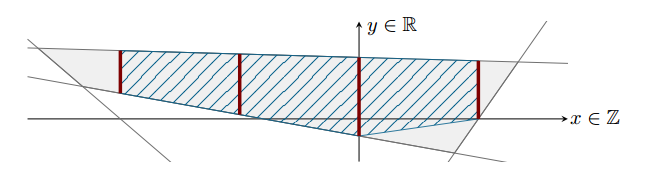
\includegraphics[width=15cm]{graphics/4-heuristic-dist/polyhedron}}
	\caption{مثالی از چند وجهی $P$ که قسمت خاکستری رنگ است و همچنین مجموعه قابل قبول جواب مسئله یعنی $P_I$ که با خطوط پررنگ قرمز مشخص شده است و مجموعه پوش محدب از جواب قابل قبول یعنی \lr{conv$(P_I)$} که ناحیه هاشور خورده آبی رنگ است. فضای استفاده شده به صورت دو بعدی است.}
	\label{fig:distributed:polyhedron}
\end{figure}
	باتوجه به نکات گفته‌شده یک مسئله خطی پیوسته در \cref{eqn:distributed:objective_func_linear} معرفی می‌کنیم که جواب بهینه‌ این مسئله با جواب بهینه مسئله \cref{eqn:distributed:objective_func} یکسان خواهد بود. به صورت شهودی با توجه به \cref{fig:distributed:polyhedron} می‌توان گفت که جواب مسئله خطی در گوشه‌های منطقه‌ قابل‌قبول\LTRfootnote{Feasible region} خواهد بود، بنابراین نقطه بهینه در این دو مسئله در نقاط مشترک خواهند بود. 
%\begin{subequations}\label{eqn:distributed:objective_func_linear}
	\begin{align}\label{eqn:distributed:objective_func_linear}
	&\min_{z}c^Tz \notag \\
	&\text{\lr{subj. to}} \quad z \in \text{\lr{conv}}(P_I) \notag \\
	&z \in \mathbb{R}^d
	\end{align}
%\end{subequations}
%todo fesible region ltrfoot
	با توجه به آن‌چه که گفته شد از این ایده برای حل کردن مسائل بهینه‌سازی خطی ترکیب عدد صحیح می‌توان استفاده کرد، به این صورت که ابتدا مسئله را به صورت خطی پیوسته در نظر می‌گیرند و هر بار یک قید جدید به مسئله اضافه می‌کنند به صورتی که فضای قابل قبول برای مسئله کوچک و کوچک‌تر شود و در نهایت با شروع از $P$ به \lr{conv$(P_I)$} رسید.
	
	در ادامه نحوه‌ی عملکرد این دسته از الگوریتم ها که به الگوریتم‌های صفحه برش\LTRfootnote{Cutting-plane} معروف هستند به صورت کلی آورده می‌شود. 
\begin{latin}
	\begin{algorithm}
		\caption{Centralized Cutting-Plane Meta-Algorithm}
		\label{alg:distributed:centralized}
		\begin{algorithmic}[1]
			\State Initialization: $ P := \bigcap_{i=1}^n \{ z \in \mathbb{R}^d : a_i^Tz \le b_i\}$
			\State LP solver: Find an optimal solution $z^{LP} = (x^{LP},y^{LP})$ of the LP relaxation of \cref{eqn:distributed:objective_func} with polyhedron P. \label{eqn:alg_steps:distributed_centralized_lp_solver}
			\State Check feasibility: if $x^{LP} \in \mathbb{Z}^{d_Z}$, go to \cref{eqn:alg_steps:distributed_centralized_last}.
			\State Cutting-Plane: $h = CUTORACLE(z^{LP},P,c)$.
			\State Update: $P := P \cap h$ and go to \cref{eqn:alg_steps:distributed_centralized_lp_solver}.
			\State Output: $z^{LP}$\label{eqn:alg_steps:distributed_centralized_last}.
		\end{algorithmic}
	\end{algorithm}
\end{latin}

	در \cref{alg:distributed:centralized} از مفهوم $CUTORACLE$ استفاده شده‌است که نشان‌دهنده یک تابع است که باتوجه به نقطه بهینه فعلی و آخرین چندوجهی مربوط به قیدها، یک قید جدید تولید می‌کند به‌طوریکه اشتراک چندوجهی قبلی و این قید جدید شامل پوش محدب مجموعه گسسته \lr{conv$(P_I)$} باشد اما شامل اخرین نقطه بهینه $z^{LP} = (x^{LP},y^{LP})$ نباشد.
	
	در ادامه لازم است که چند مفهوم دیگر تعریف شود. یک جعبه مجدود به صورت \cref{eqn:distributed:bounding_box} تعریف می‌شود که در ادامه از آن استفاده خواهد شد. فرض می‌شود که $P \subset H_M$.
\begin{equation}\label{eqn:distributed:bounding_box}
H_M := \bigcap_{l=1}^d (\{ z_l \le M \} \cap \{ z_l \ge -M \})
\end{equation}
	یک مفهوم دیگر به نام پایه\LTRfootnote{Basis} تعریف می‌شود، فرض کنید که یک مسئله بهینه‌سازی خطی پیوسته با مجموعه قید $P := \bigcap_{i=1}^n P_i$ داریم که هریک از $P_i$ ها یک نیم‌فضا\LTRfootnote{Half-spce} است، پایه $B$ مجموعه‌ تشکیل شده از تقاطع حداقل تعداد نیم‌فضا $P_{l_1}, \dots, P_{l_q}$ است به صورتی‌که $q \le d$ و جواب بهینه مسئله بهینه سازی بر روی مجموعه قید $P$ با جواب همان مسئله بر روی مجموعه قید $B$ برابر است. اگر برای حل کردن مسئله بهینه‌سازی از الگوریتم $LEXOPTIMAL$ که نوعی الگوریتم سیمپلکس\LTRfootnote{Simplex} است استفاده شود، می‌توان نشان داد که $B$ دقیقا از تقاطع $d$ نیم‌فضا تشکیل می‌شود.  الگوریتم $LEXOPTIMAL$ به تفصیل در \cite{jones2007lexicographic} توضیح داده شده‌است.
	%todo lexoptimal cite
	
\begin{latin}
	\begin{algorithm}
		\caption{Distributed Meta-Algorithm}
		\label{alg:distributed:int_distributed}
		\begin{algorithmic}[1]
			\Statex State $(z^{[i]},B^{[i]})$
			\Statex Initializing    
			\State $h^{[i]} = h_{i0} \cap H_M$
			\State $(z^{[i]},B^{[i]}) = LPLEXSOLV(h^{[i]}, c)$
			\Statex Evolution 
			\State $(h_{MIG}(t),h_c(t)) = CUTORACLE(z^{[i]}(t),B^{[i]}(t),c)$
			\State $\displaystyle H_{TMP}(t) = (\bigcap_{j \in N_i(t)}B^{[j]}(t)) \cap B^{[i]}(t) \cap h^{[i]} \cap h_{MIG}(t) \cap h_c(t)$
			\State $(z^{[i]}(t+1),B^{[i]}(t+1)) = LPLEXSOLV(H_{TMP}, c)$
		\end{algorithmic}
	\end{algorithm}
\end{latin}
%todo h_mig H_M
در \cref{alg:distributed:int_distributed} خروجی تابع CUTORACLE به‌صورت دو قسمتی است. که لازم است در مورد آن صحبت شود. در \cite{gomory1960algorithm} یک روش برش به نام MIG\LTRfootnote{Mixed-Integer Gomory} ارائه شده است و اثبات شده است که در صورتی‌که تابع هدف مسئله بهینه‌سازی به صورت گسسته باشد، این روش صفحه برش می‌تواند مسئله را حل کند. خروجی تابع که به صورت $h_{MIG}$ نشان داده شده‌است، مربوط به این نحوه‌ی برش می‌باشد. خروجی دیگر که با نماد $h_c$ نشان داده شده‌است در \cref{eqn:distributed:cost_based_cut} آورده شده‌است. 
\begin{align}\label{eqn:distributed:cost_based_cut}
	h_c = \{ c^Tz > \lceil c^Tz^{LP}\rceil \}	
\end{align}
	بنابراین از \cref{alg:distributed:int_distributed} برای حل کردن مسئله خطی ترکیب عددصحیح به‌صورت کاملا توزیع‌شده استفاده می‌شود، اما این شرط اساسی وجود دارد که تابع هدف مسئله بهینه‌سازی به صورت گسسته(عددصحیح) باشد. 
	برای حل مشکل شرط گسسته بودن تابع هدف یک الگوریتم دیگر ارائه می‌شود که در \cref{alg:distributed:epsilon_distributed} آورده شده‌است. ابتدا مسئله اصلی نوشته شده در \cref{eqn:distributed:objective_func} به صورت \cref{eqn:distributed:objective_func_epigraph} بازنویسی می‌شود، که مدل epigraph نامیده می‌شود. 
	\begin{subequations}\label{eqn:distributed:objective_func_epigraph}
		\begin{align}
		&\min_{\rho,z}\rho \\
		&\text{\lr{subj. to}} \quad a_i^Tz \le b_i, i = 1, \dots, n  \\
		&c^Tz \le \rho \\
		&\rho \in \mathbb{R}, z \in \mathbb{Z}^{d_Z} \times \mathbb{R}^{d_R} \\
		\end{align}
	\end{subequations}
	حال می‌دانیم که $\rho$ لزوما به صورت عددصحیح نیست، بنابراین یک متغیر دیگر به نام $\rho_I$ که فرض می‌کنیم به صورت عددصحیح است، به‌صورت $\epsilon\rho_I = \rho$ تعریف می‌شود. حال مسئله بهینه‌سازی مجددا به فرم \cref{eqn:distributed:objective_func_epigraph_int} بازنویسی می‌شود و درنهایت الگوریتم توزیع‌شده برای این مسئله نوشته می‌شود. 
	\begin{subequations}\label{eqn:distributed:objective_func_epigraph_int}
		\begin{align}
		&\min_{\rho_I,z}\rho_I \\
		&\text{\lr{subj. to}} \quad a_i^Tz \le b_i, i = 1, \dots, n  \\
		&c^Tz \le \epsilon \rho_I \\
		&\rho_I \in \mathbb{Z}, z \in \mathbb{Z}^{d_Z} \times \mathbb{R}^{d_R}, \epsilon > 0 \\
		\end{align}
	\end{subequations}
	درنهایت می‌توان \cref{alg:distributed:epsilon_distributed} را به‌صورت زیر نوشت که برای تمام مسئله‌های خطی ترکیب عددصحیح جواب می‌دهد. توضیح بیشتر درمورد چزئیات این الگوریتم این‌که هریک از گره‌ها قید اولیه و محلی خود را به صورت $h_{i0} = \{ a_i^Tz \le b_i\} \cap \{c^Tz \le \epsilon\rho\}$ در نظر می‌گیرد. زوج متغیر $\rho_I$ , $z$ را نیز به عنوان هزینه جدید درنظر می‌گیرم و با $e_1$ نشان می‌دهیم. 
\begin{latin}
	\begin{algorithm}
		\caption{Distributed Algorithm}
		\label{alg:distributed:epsilon_distributed}
		\begin{algorithmic}[1]
			\Statex State $((\rho_I^{[i]},z^{[i]}),B^{[i]})$
			\Statex Initializing    
			\State $h^{[i]} = h_{i0} \cap H_M$
			\State $((\rho_I^{[i]},z^{[i]}),B^{[i]}) = LPLEXSOLV(h^{[i]}, e_1)$
			\Statex Evolution 
			\State $h_{MIG}(t) = MIGORACLE((\rho_I^{[i]}(t),z^{[i]}(t)),B^{[i]}(t),c)$
			\State $h_c(t) = \{ \rho_I \ge \lceil\rho_I^{[i]}(t)\rceil \} $
			\State $\displaystyle H_{TMP}(t) = (\bigcap_{j \in N_i(t)}B^{[j]}(t)) \cap B^{[i]}(t) \cap h^{[i]} \cap h_{MIG}(t) \cap h_c(t)$
			\State $((\rho_I^{[i]}(t+1),z^{[i]}(t+1)),B^{[i]}(t+1)) = LPLEXSOLV(H_{TMP}, e_1)$
		\end{algorithmic}
	\end{algorithm}
\end{latin}

در هر دو الگوریتم ارائه شده، هر گره متغیر اصلی مسئله را به صورت محلی ذخیره می‌کند و در هر مرحله بعد از تبادل اطلاعات با همسایه‌های خود و دریافت قید(برش)های جدید، متغیر اصلی مسئله را بروز رسانی می‌کند. سوالی که پیش می‌آید، این است که هر گره از کجا بداند فرآیند حل مسئله تمام شده است یا نه، در \cite{testa2019distributed} گفته شده‌است که هروقت یک گره از تمام همسایه‌های خود هیچ قید جدیدی دریافت نکرد، این بدین معنی است که فرآیند حل مسئله به پایان رسیده است. 

	در این قسمت لازم است که مسئله این پایان‌نامه را به فرم \cref{eqn:distributed:objective_func} و سپس \cref{eqn:distributed:objective_func_epigraph} بنویسم. ابتدا لازم است که متغیر اصلی یعنی $z$ را تعریف کنیم، که در \cref{eqn:distributed:def_z} انجام شده‌است. 
\begin{subequations}\label{eqn:distributed:def_z}
	\begin{align}
		&z = (\underline{x_e}^T, \underline{x_f}^T, \underline{x_c}^T, \underline{\underline{\beta_{e}}}(:)^T, \underline{\underline{\beta_{f}}}(:)^T, \underline{\underline{\beta_{c}}}(:)^T)^T \\
		&\underline{x_e} = (x_{e,1}, \dots, x_{e,|T|})^T \\
		&[\underline{\underline{\beta_{e}}}]^i_j = \beta_{i,j,e}
	\end{align}
\end{subequations}
%todo matrix elements syntax and all elements of a matrix in a row syntax
در قدم بعدی لازم است که قیدها را بین گره‌ها تقسیم کنیم، در مورد قیدهای مسئله اصلی که تفکیک‌پذیر هستند، یعنی قیدهای \cref{eqn:constraint_load_conservation_computing_nodes}، \cref{eqn:constraint_request_flow_existence}،\cref{eqn:constraint_psi} ، \cref{eqn:constraint_load_managing_linear}، \cref{eqn:constraint_delay_linear} و \cref{eqn:constraint_queue_stability_linear} وضعیت مشخص است، اما در مورد دو قید \cref{eqn:constraint_scalability_coupling} و \cref{eqn:constraint_load_conservation_sensor_nodes_coupling_new2} که به صورت مشترک هستند لازم است تصمیم گرفته‌شود. تعداد قیدهای دسته اول $|T|$ تاست و تعداد قیدهای دسته دوم $|T| \times |S|$ تاست، در حالی‌که تعداد گره‌های پردازشی از \cref{eqn:def_globals} مشخص می‌شود. حال لازم است که این دودسته قید بین گره‌ها توزیع شوند، برای توزیع بهتر می‌توان از این ایده کمک گرفت که توزیع قیدها را از گره‌هایی که توانایی پردازش بیشتری دارند شروع کرد. به‌صورت میانگین به هر گره $\frac{|T|\times(|S|+1)}{l}$ قید می‌رسد. در نهایت $\rho$ به راحتی با مقایسه با تابع هدف در \cref{eqn:objective_func}

\section{بررسی همگرایی و پیچیدگی}
	در این بخش نوع همگرایی و میزان پیچیدگی دو الگوریتم گفته شده در این فصل مورد بررسی قرار می‌گیرد. 
	در \cite{testa2019distributed} نویسندگان اثبات کرده‌اند که \cref{alg:distributed:epsilon_distributed} جوابه شبه بهینه ارائه می‌دهد. 
	در این منبع در مورد میزان پیچیدگی الگوریتم توزیع‌شده نیز اشاره شده‌است که این الگوریتم در زمان خطی نسبت به توپولوژی مسئله(مثلا تعداد گره‌ها یا ...) به جواب می‌رسد. 
	
	در مورد روش اکتشافی ارائه شده نیز می‌توان گفت با فرض اینکه تعداد کل وظیفه‌ها $|T|$ باشد و تعداد کل گره‌های محاسباتی $l$ باشد، همچنین حداکثر تعداد قابل تقسیم برای هر وظیفه $N_t$ باشد. آنگاه میزان پیچیدگی محاسباتی برای یافتن جواب به کمک روش جستجو اکتشافی از حدود $O(l\times(|T|N_t)^2)$ خواهد بود که نسبت به ابعاد مسئله خطی است. 
	
\section{نتایج شبیه‌سازی}

\begin{figure}[h!]
	\centerline{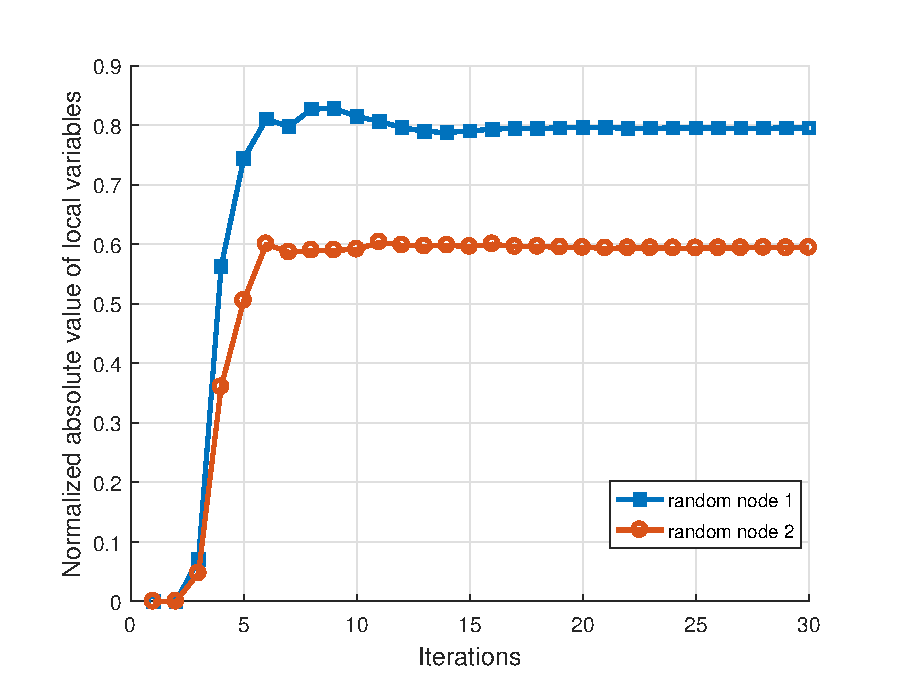
\includegraphics[width=12cm]{graphics/4-heuristic-dist/distributed_local_vars_convergence}}
	\caption{نحوه‌ همگرا شدن متغیر محلی در دو گره تصادفی در روش توزیع‌شده}
	\label{fig:distributed_local_vars_convergence}
\end{figure}

	دراین بخش نتایج شبیه‌سازی‌های مربوط به این فصل آورده شده‌است. ابتدا نحوه‌ی همگرایی در روش توزیع شده را بررسی می‌کنیم. در \cref{fig:distributed_local_vars_convergence} نحوه همگرایی برای دو گره تصادفی از شبکه در روش توزیع شده به نمایش گذاشته شده‌است. در این نمودار اندازه متغیر محلی برای این دوگره در طول زمان نشان داده شده‌است. 
	
\begin{figure}[h!]
	\centerline{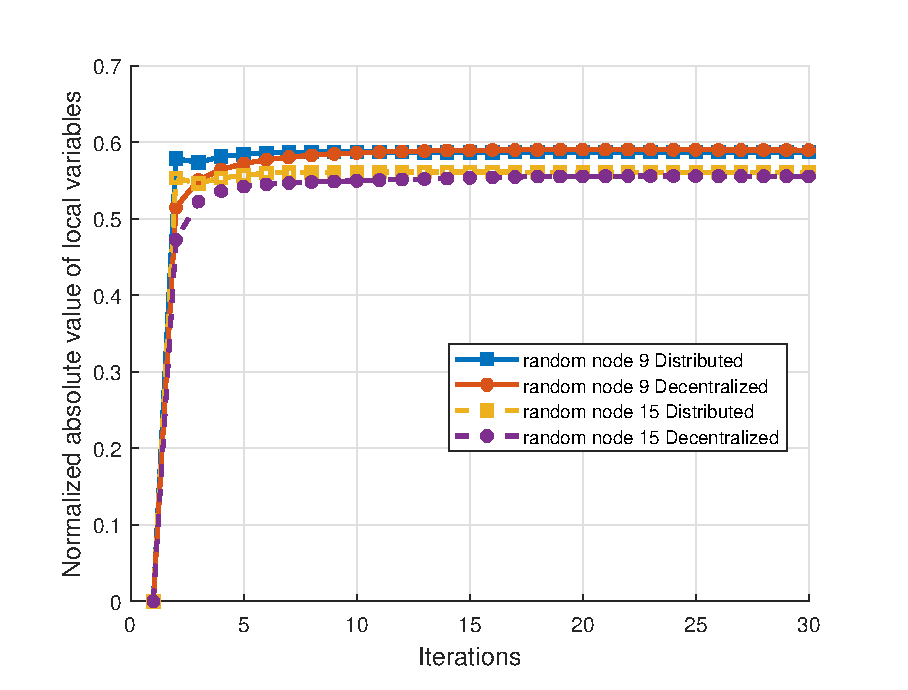
\includegraphics[width=12cm]{graphics/4-heuristic-dist/distributed_decent_local_vars_convergence}}
	\caption{نحوه‌ همگرا شدن اندازه‌ی متغیر  محلی مسئله در دو روش توزیع‌شده و غیرمتمرکز برای دوگره تصادفی}
	\label{fig:distributed_decent_local_vars_convergence}
\end{figure}

	در \cref{fig:distributed_decent_local_vars_convergence}	نحوه‌ همگرایی متغیر محلی در دو روش غیرمتمرکز و توزیع‌شده مقایسه شده‌است. همانطور که دیده می‌شود در روش غیرمتمرکز سرعت همگرایی اندکی بیشتر است، که دلیل آن وجود واحد هدایت‌گر\LTRfootnote{Coordinator} در روش غیرمتمرکز است که باعث می‌شود سرعت همگرایی بیشتر شود و همچنین نحوه همگرایی صاف‌تر باشد. 

\begin{figure}[h!]
	\centerline{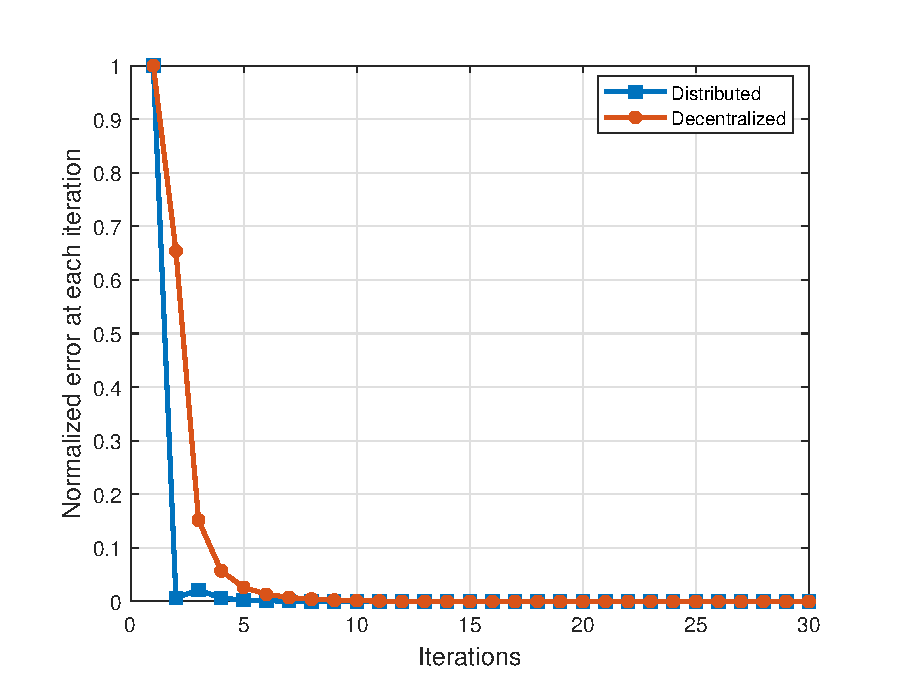
\includegraphics[width=12cm]{graphics/4-heuristic-dist/error_convergence_dist_decent}}
	\caption{نحوه همگرا شدن مقدار خطا در دو روش توزیع‌شده و غیرمتمرکز}
	\label{fig:error_convergence_dist_decent}
\end{figure}

	در \cref{fig:error_convergence_dist_decent} نیز نحوه همگرایی میزان خطا در دو روش غیرمتمرکز و توزیع‌شده به نمایش گذاشته شده‌است. در این نمودار در هر مرحله اختلاف مقدار تابع هدف با مرحله قبل به صورت خطا در نظر گرفته شده‌است که این خطا به صورت یکه شده نمایش داده شده‌است. 

\begin{figure}[h!]
	\centerline{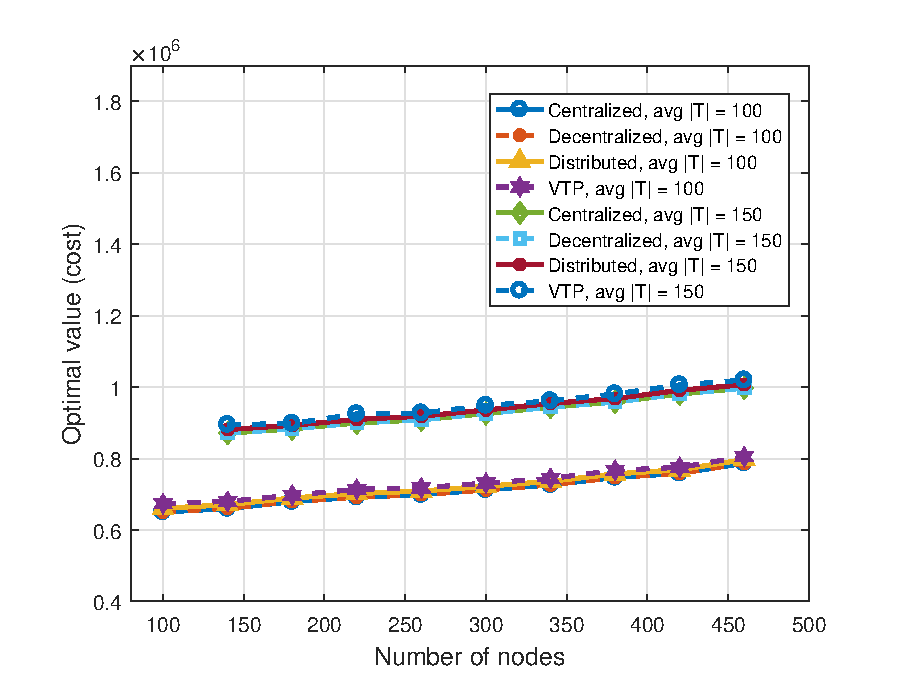
\includegraphics[width=12cm]{graphics/4-heuristic-dist/optimization_value_per_number_of_nodes_all_solutions}}
	\caption{مقدار تابع هدف (هزینه) برای چهار روش مختلف دربرابر تعداد کل گره‌های شبکه}
	\label{fig:optimization_value_per_number_of_nodes_all_solutions}
\end{figure}

	در شبیه‌سازی بعدی هر چهار روش موجود بر روی شبکه اجرا شده‌است، در این شبیه‌سازی سعی شده است که در هر مرحله تمام پارامترهای موجود در شبکه به صورت تصادفی انتخاب شود که این تصادفی بود در \cref{fig:optimization_value_per_number_of_nodes_all_solutions} به‌خوبی دیده  می‌شود. همانطور که از این نمودار دیده می‌شود مقدار تابع هدف در دو راه‌جل متمرکز و غیرمتمرکز بهینه است و در راه حل توزیع‌شده نیز با فاکتور دلخواه $\epsilon$ قابل کنترل است، اما در مورد راه‌حل اکتشافی می‌بینیم که این راه‌حل جواب شبه بهینه را می‌دهد. 
\begin{figure}[h!]
	\centerline{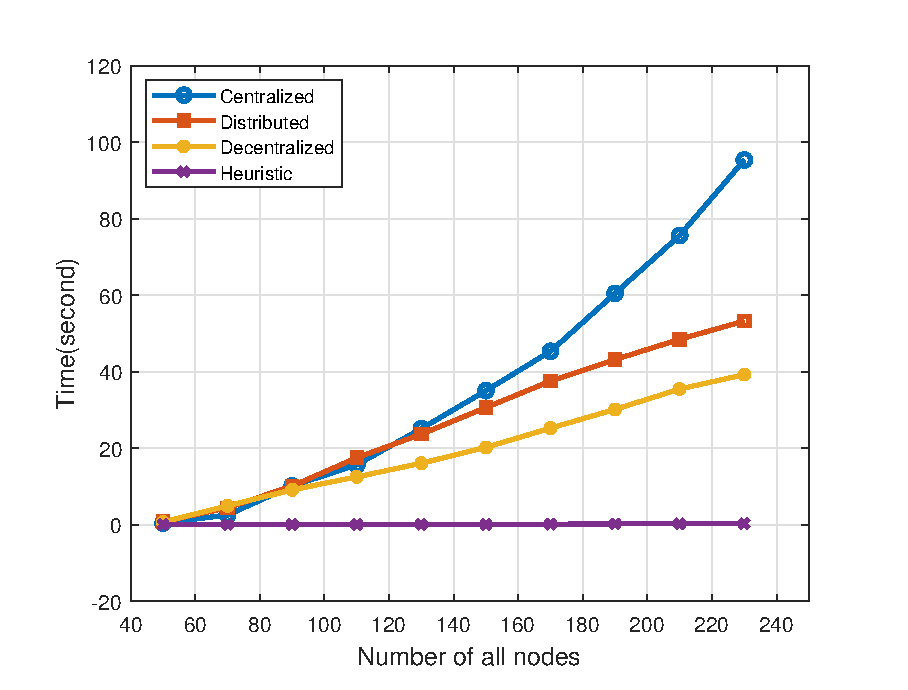
\includegraphics[width=12cm]{graphics/4-heuristic-dist/time_of_convergence}}
	\caption{مدت زمان آماده شدن جواب نهایی در چهار روش مختلف دربرابر تعداد کل گره‌های شبکه}
	\label{fig:time_of_convergence}
\end{figure}

	آخرین تحلیل مربوط به زمان آماده شدن جواب در چهار راه‌حل ارائه‌شده در این پایان‌نامه است. سعی شده است که شبیه‌سازی‌ها در شرایط کاملا یکسان انجام شود، ازجمله میزان حافظه موجود بر روی دستگاه کامپیوتری که تست ها برروی انجام شده‌است و یا دمای پردازنده در هنگام تست و ... . همانطور که دیده می‌شود به وضوح زمان انجام محاسبات در راه‌حل اکتشافی کم است. در مورد دو راه حل غیرمتمرکز و توزیع‌شده نیز ذکر این نکته لازم است که شرایط واقعی شبیه‌سازی زمانی‌است که محاسبات در گره‌های مختلف و بهٍٍ‌صورت همزمان انجام شود در حالیکه در تست‌های انجام شده به دلیل محدودیت منابع کلیه شبیه‌سازی‌ها بر روی یک دستگاه انجام شده‌است که این خود باعث می‌شود خاصیت اصلی این دو روش به خوبی دیده نشود، که با این وجود در \cref{fig:time_of_convergence} تقریبا دیده می‌شود که آماده شدن جواب در سه روش غیرمتمرکز، توزیع‌شده و اکتشافی به صورت خطی نسبت به اندازه توپولوژی مسئله است. 
	
	\section{جمع‌بندی و نتیجه‌گیری}
	در این فصل دو روش دیگر برای حل مسئله اصلی ارائه‌شد. روش اول یک روش کاملا توزیع شده است که مسئله بین تمام گره‌های پردازشی تقسیم می‌شود و از قدرت پردازشی آن‌ها برای حل مسئله کمک گرفته می‌شود. روش دوم نیز یک راه‌حل اکتشافی بود که مسئله اصلی را بدون نیاز به خطی‌سازی و به صورت اکتشافی حل می‌کند. هردو روش ارائه شده در این فصل جواب شبه‌بهینه ارائه می‌کردند. 
	در قسمت نتایج دیده شد که هر دوروش در زمان خطی به نتیجه می‌رسند و چهار روش ارائه شده در این پایان‌نامه با یکدیگر مقایسه شد. 

